\section{Dataset}
\label{sec:dataset}
The dataset consists of books from the 16\textsuperscript{th} and
17\textsuperscript{th} century, which were downloaded from Google Books.
\begin{comment}
%Moved to annotator part of this section
There are several peculiarities. Table
\ref{tab:statistics} shows that the amount of pages per book, and the amount of
images per book differs enormously per book.
\end{comment}
Some examples of the pages can be seen in figure \ref{fig:textImageExamples},
\ref{fig:textExamples}, \ref{fig:imageExamples}, \ref{fig:qualityExamples} and
\ref{fig:baggerExamples}. Figure \ref{fig:qualityExamples} shows that there is
quite a large gap between the quality of scans of some books. The right image of
figure \ref{fig:qualityExamples}
has a vertical line, which indicates that parts of both pages were scanned into the same
image. Furthermore, figure \ref{fig:baggerExamples} shows that some pages
contain something that we can neither classify as text nor as an image.

\begin{table}
\centering
\begin{tabular}{@{\extracolsep{4pt}}l r r @{}}
\hline
 & \textbf{Training set} & \textbf{Test set}\\\hline
\textbf{Total amount of pages:} & 5960 & 2868\\
\textbf{Mean pages per book:} & 236 & 717\\
\textbf{Standard deviation:} & 223 & 290\\
\hline
\textbf{Total amount of images:} & 525 & 286 \\
\textbf{Mean images per book:} & 22.8 & 71.5\\
\textbf{Standard deviation:} & 49.8 & 61.6\\\hline
\end{tabular}
\caption{Dataset statistics}
\label{tab:statistics}
\end{table}

% Give the images some space!
\newgeometry{margin=3cm}
\begin{figure}[H]
	\centering
	\begin{subfigure}[b]{0.49\textwidth}
		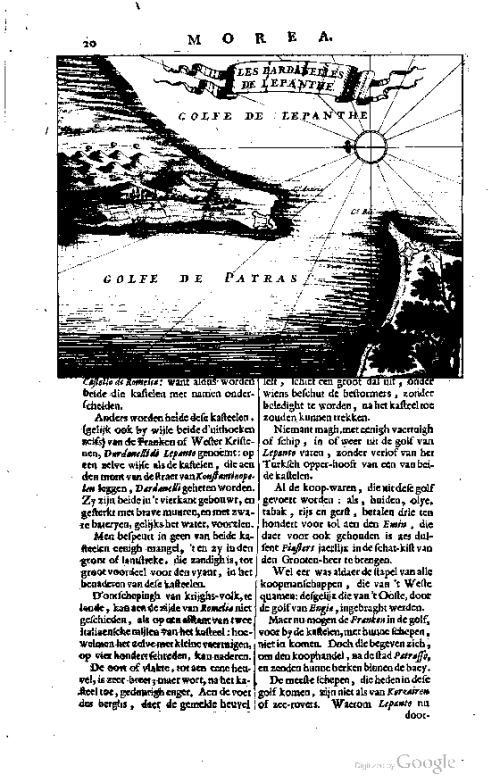
\includegraphics[width=.49\textwidth]{resources/pageImageExample}
		
\includegraphics[width=.49\textwidth]{resources/pageImageExample2}
		\caption{Examples of pages that contain both text and images}
		\label{fig:textImageExamples}
	\end{subfigure}
	\begin{subfigure}[b]{0.49\textwidth}
		
\includegraphics[width=.49\textwidth]{resources/500_0043}
		
\includegraphics[width=.49\textwidth]{resources/500_0010}
		\caption{Examples of pages that consist of text}
		\label{fig:textExamples}
	\end{subfigure}
	\begin{subfigure}[b]{0.49\textwidth}
		
\includegraphics[width=.49\textwidth]{resources/500_0008}
		
\includegraphics[width=.49\textwidth]{resources/500_0077}
		\caption{Examples of pages that consist of images}
		\label{fig:imageExamples}
	\end{subfigure}
	\begin{subfigure}[b]{0.49\textwidth}
		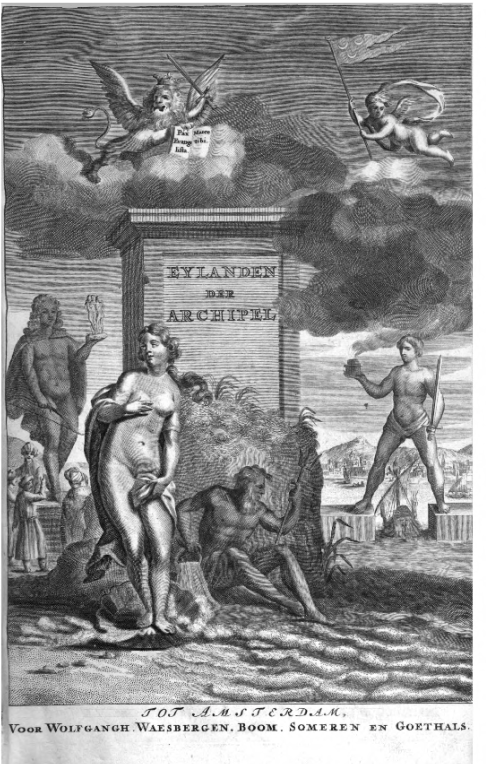
\includegraphics[width=.49\textwidth]{resources/good_quality}
		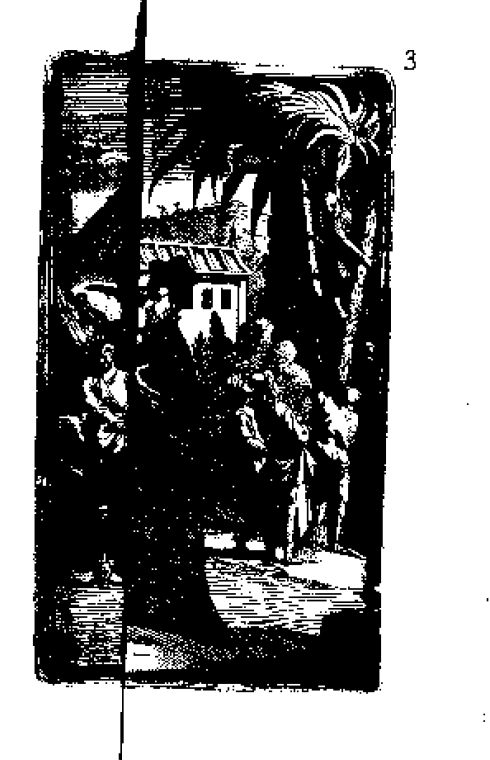
\includegraphics[width=.49\textwidth]{resources/bad_quality}
		\caption{The quality differs per book}
		\label{fig:qualityExamples}
	\end{subfigure}
	\begin{subfigure}[b]{0.49\textwidth}
		
\includegraphics[width=.49\textwidth]{resources/500_0002}
		
\includegraphics[width=.49\textwidth]{resources/500_0004}
		\caption{Some pages contain neither text nor image}
		\label{fig:baggerExamples}
	\end{subfigure}
	\caption{Examples of book pages from the dataset\todo{Fix the new page that
	occurs before this figure}}
	\label{fig:examples}
\end{figure}
\restoregeometry

